%============================================================%
\documentclass[a4paper,12pt]{article}
%%%%%%%%%%%%%%%%%%%%%%%%%%%%%%%%%%%%%%%%%%%%%%%%%%%%%%%%%%%%%%%%%%%%%%%%%%%%%%%%%%%%%%%%%%%%%%%%%%%%%%%%%%%%%%%%%%%%%%%%%%%%%%%%%%%%%%%%%%%%%%%%%%%%%%%%%%%%%%%%%%%%%%%%%%%%%%%%%%%%%%%%%%%%%%%%%%%%%%%%%%%%%%%%%%%%%%%%%%%%%%%%%%%%%%%%%%%%%%%%%%%%%%%%%%%%
\usepackage{eurosym}
\usepackage{vmargin}
\usepackage{amsmath}
\usepackage{graphics}
\usepackage{epsfig}
\usepackage{subfigure}
\usepackage{fancyhdr}
\usepackage{listings}
\usepackage{framed}
\usepackage{graphicx}
\usepackage{amsmath}
\usepackage{chngpage}
%\usepackage{bigints}


\setcounter{MaxMatrixCols}{10}

\begin{document}
	\begin{center}
		
\includegraphics[scale=0.55]{images/shieldtransparent2}
	\end{center}
	
	\begin{center}
		\vspace{1cm}
		\large \bf {FACULTY OF SCIENCE AND ENGINEERING} \\[0.5cm]
		\normalsize DEPARTMENT OF MATHEMATICS AND STATISTICS \\[1.25cm]
		\large \bf {END OF SEMESTER EXAMINATION PAPER 2015} \\[1.5cm]
	\end{center}
	
	\begin{tabular}{ll}
		MODULE CODE: MA4505 & SEMESTER: Autumn 2015 \\[1cm]
		MODULE TITLE: Applied Statistics & DURATION OF EXAM: 2.5 hours  \\
		\phantom{MODULE TITLE:} For Administration 1 & \\ [1cm]
		LECTURER: Mr. Kevin O'Brien & GRADING SCHEME: 100 marks \\
		& \phantom{GRADING SCHEME:} \footnotesize {70\% of module grade} \\[1cm]
EXTERNAL EXAMINER: Prof. J. King & \\
	\end{tabular}
\vspace{0.3cm}
	\begin{center}
		{\bf INSTRUCTIONS TO CANDIDATES}
	\end{center}
	
	{\noindent \\ Scientific calculators approved by the University of Limerick can be used. \\
		Formula sheet and statistical tables provided at the end of the exam paper.\\
		There are 5 questions in this exam. Students must attempt any 4 questions.}
	%====================================================================== %
	\newpage
	\subsection*{Question 1 Inference Procedures}
	
%	\begin{framed}
%		What is going here?
%		\begin{itemize}
%			\item Using the Murdoch Barnes Table for Normal Distribution Problems
%			\item Testing that Data is normally distributed (may appear elsewhere)
%			\item Transformation of Data (Tukey's Ladder)
%			\item Outliers and Boxplots (Grubbs Test, Dixon Q-test)
%			\item Non-Parametric Procedures (e.g. Wilcoxon test, Kolmogorov Smirnov Test)
%		\end{itemize}
%	\end{framed}
%\newpage
%\subsubsection*{Question 1 Part A (4 Marks)}
%%\subsubsection*{Part A Theory for Inference Procedures (4 Marks)}
%Answer the four short questions. Each correct answer will be awarded 1 mark.
%\begin{itemize}
%	\item[(i.)] What is a $p-$value?
%	\item[(ii.)] Briefly describe how $p-$value is used in hypothesis testing.
%	\item[(iii.)] What is meant by a Type I error?
%	\item[(iv.)] What is meant by a Type II error?
%\end{itemize}
\subsubsection*{Question 1 Part A (5 Marks)}
Numeric Transformations, such as logarithmic transformation, are often used in statistical analysis as an approach for dealing with non-normal data.
\begin{itemize}
	%	\item[(i)] (1 Marks) Discuss the importance of numeric transformations, such as logarithmic transformation, in Statistics.
	%	\item[(ii)] Describe the process of transformations
	\item[(i.)] (1 Mark) Describe the purpose of Tukey's Ladder (referencing direction and relative strength).
	\item[(ii.)] (2 Marks) Give two examples of a transformation for various types of skewed data (i.e. an example for both types of skewness).
	\item[(iii.)] (1 Mark) Discuss the limitations of numeric transformations.
\end{itemize}
\bigskip

\subsubsection*{Question 1 Part B (5 Marks)}

The typing speeds for one group of 12 Engineering students were recorded both at the beginning of year 1 of their studies. The results (in words per minute) are given below:

\begin{center}
	\begin{tabular}{|c|c|c|c|c|c|}
		\hline
		% Subject& A& B& C& D& E &F &G &H \\ \hline
		149  & 146 & 112 & 142 & 168& 153\\ \hline
		137 & 161 & 156& 165&  170&  159
		\\ \hline
	\end{tabular}
\end{center}
Use the Dixon Q-test to determine if the lowest value (118) is an outlier. You may assume a significance level of 5\%.
\begin{itemize}
	\item[(i.)](1 Mark)	State the Null and Alternative Hypothesis for this test.
	\item[(ii.)](2 Marks) Compute the test statistic
	\item[(iii.)](1 Mark) State the appropriate critical value.
	\item[(iv.)](1 Mark) What is your conclusion to this procedure.
\end{itemize}
\newpage
\subsubsection*{Question 1 Part C (5 Marks)}

%\subsubsection*{Part A : Outliers}
\begin{itemize}
	\item[(i.)] (3 Marks) Provide a brief description for three tests from the family of Grubb's  Outliers Tests. Include in your description a statement of the null and alternative hypothesis for each test
	\item[(ii.)] (2 Marks) Describe any required assumptions for tests, and the limitations of these tests.
\end{itemize}



% Review of Univariate Normal Distribution
% Test for Univariate normality
% - Graphical Procedures
% - Formal Tests
% (Later Multivariate Normality)
% Boxplots, Outliers and Transformations
%
% (Hint: there are no outliers in these data sets)

\bigskip
%--------------------------------------------------------------------------------------- %
\subsubsection*{Question 1 Part D (10 Marks)}
% Normal %6 MARKS
Assume that the diameter of a critical component is normally distributed with a mean of 250mm and a standard deviation of 15mm. You are required  to estimate the approximate probability of the following measurements occurring on an individual component.
\begin{itemize}
	\item[(i.)](3 Mark) Greater than 245mm.
	\item[(ii.)](3 Marks) Less than 265mm.
	\item [(iii.)](4 Marks) Between 245mm and 265mm.
\end{itemize}
\bigskip
\noindent Use the normal tables to determine the probabilities for the above exercises. You are required to show all of your workings.


	%====================================================================== %
	\newpage
\subsection*{Question 2 Chi-Squared and One-Way ANOVA F-test}
\subsubsection*{Question 2 Part A (13 Marks)}

A market research survey was carried out to assess preferences for three brands of chocolate bar, A, B, and C. 
The study group was categorised by gender to determine any difference in preferences.


{
	\large
	\begin{center}
		\begin{tabular}{|c|c|c|c|c|}
			\hline
			& X & Y & Z &  Total\\ \hline
			Children  & 50 & 70 & 80 & 200 \\ \hline
			Teenagers  & 90 & 50 & 20 &  160\\ \hline
			Adults  & 140 & 120 & 100 & 360\\ \hline
		\end{tabular} 
	\end{center}
}
\begin{itemize}
	\item[(i.)](2 Mark) Formally state the null and alternative hypotheses.
	\item[(ii.)] (4 Marks) Compute the cell values expected under the null hypothesis. 
	\item[(iii.)](4 Marks) Compute the test statistic.
	\item[(iv.)](2 Mark) State the appropriate critical value for this hypothesis test.
	\item[(v.)](3 Mark) Discuss your conclusion to this test, supporting your statement with reference to appropriate values.
\end{itemize}
\newpage
\subsubsection*{Question 2 Part B (6 Marks)}
Six analysts each made seven determinations of the paracetamol content of the same batch of tablets.
The results are shown below. There are 42 determinations in total. The mean determination for each analysts is also tabulated. \\


%Analyst= structure(c(1L, 2L, 3L, 4L, 5L, 6L, 1L, 2L, 3L, 4L, 5L, 6L, 1L,
%2L, 3L, 4L, 5L, 6L, 1L, 2L, 3L, 4L, 5L, 6L, 1L, 2L, 3L, 4L, 5L,
%6L, 1L, 2L, 3L, 4L, 5L, 6L, 1L, 2L, 3L, 4L, 5L, 6L), .Label = c("A",
%"B", "C", "D", "E", "F"), class = "factor")

%Determinations= c(84.32, 84.24, 84.29, 84.14, 84.5, 84.7, 84.61, 84.13, 84.28,
%84.48, 83.91, 84.36, 84.64, 84, 84.4, 84.27, 84.11, 84.61, 84.62,
%84.02, 84.63, 84.22, 83.99, 84.15, 84.51, 84.25, 84.4, 84.22,
%83.88, 84.17, 84.63, 84.41, 84.68, 84.02, 84.49, 84.11, 84.51,
%84.3, 84.36, 84.33, 84.06, 83.81)

\begin{center}
	\begin{tabular}{|c|ccccccc|}
		\hline
		Analyst	& Content		&		&		&		&		&		&		 \\ \hline
		A	&	84.32	&	84.61	&	84.64	&	84.62	&	84.51	&	84.63	&	84.51	 \\
		B	&	84.24	&	84.13	&	84.00	&	84.02	&	84.25	&	84.41	&	84.30	 \\
		C	&	84.29	&	84.28	&	84.40	&	84.63	&	84.40	&	84.68	&	84.36	 \\
		D	&	84.14	&	84.48	&	84.27	&	84.22	&	84.22	&	84.02	&	84.33	 \\
		E	&	84.50	&	83.91	&	84.11	&	83.99	&	83.88	&	84.49	&	84.06	 \\
		F	&	84.70	&	84.36	&	84.61	&	84.15	&	84.17	&	84.11	&	83.81	 \\
		\hline
	\end{tabular}
\end{center}
\bigskip
The following \texttt{R} output has been produced as a result of analysis of these data:

%Experiment=data.frame(Determinations, Analyst)
%Model=aov(Determinations~Analyst)
%summary(Model)

%Analysis of Variance Table
%
%            Df Sum Sq Mean Sq F value  Pr(>F)
%Analyst      5 0.8611 0.17222   4.236 0.00394 **
%Residuals   36 1.4635 0.04065
%---
%Signif. codes:  0 ‘***’ 0.001 ‘**’ 0.01 ‘*’ 0.05 ‘.’ 0.1 ‘ ’ 1

\begin{center}
	\texttt{
		\begin{tabular}{|cc|c|c|c|c|c|}
			\hline
			% after \\: \hline or \cline{col1-col2} \cline{col3-col4} ...
			&&		&		&		&		&		\\
			Response: Y        	&&	Df  	&	Sum Sq 	&	Mean Sq 	&	F value    	&	$Pr(>F)$    	\\
			&&	\phantom{make}	&		&		&		&		\\\hline \hline
			&&		&	\phantom{make}	&		&		&		\\
			Analyst 	&&	\textbf{?}	&	\textbf{?}	&	\textbf{?}	&	\textbf{?}	&	0.00394 **	\\
			&&		&		&		&		&		\\ \hline
			&&		&		&		&		&		\\
			Residuals	&&	\textbf{?}	&	\textbf{?}	&	0.04065	&	&		\\
			&&		&		&		&		&		\\ \hline
			&&		&		&		&		&		\\
			Total	&&	\textbf{?}	&	2.3246	&		&		&		\\
			&&		&		&		&		&		\\ \hline
		\end{tabular}
	}
\end{center}
\begin{itemize}
	\item[(i.)] (6 Marks) Complete the ANOVA table in your answer sheet, replacing the "?" entries with the correct values.\textit{\\ (You are not required to carry out a hypothesis test.)}
%	\item[ii.] (2 marks) What hypothesis is being considered by this procedure.

\end{itemize}
\newpage
\subsubsection*{Question 2 Part C (7 Marks)}
The \texttt{R} code and graphical procedures, below and on the following page, are relevant to checking whether the underlying assumptions are met for the ANOVA model in part (b).
\begin{itemize}
	\item[(i.)] (3 marks) What are the assumptions underlying ANOVA?
	\item[(ii.)] (4 marks)  Assess the validity of these assumptions for the ANOVA model in Part B.
	
\end{itemize}
\begin{framed}
	\begin{verbatim}
	Shapiro-Wilk normality test
	
	data:  Residuals
	W = 0.9719, p-value = 0.3819
	\end{verbatim}
\end{framed}
\begin{framed}
	\begin{verbatim}
	Bartlett test of homogeneity of variances
	
	data:  Experiment
	Bartlett's K-squared = 105.9585, df = 1, p-value < 2.2e-16
	\end{verbatim}
\end{framed}
\begin{center}
	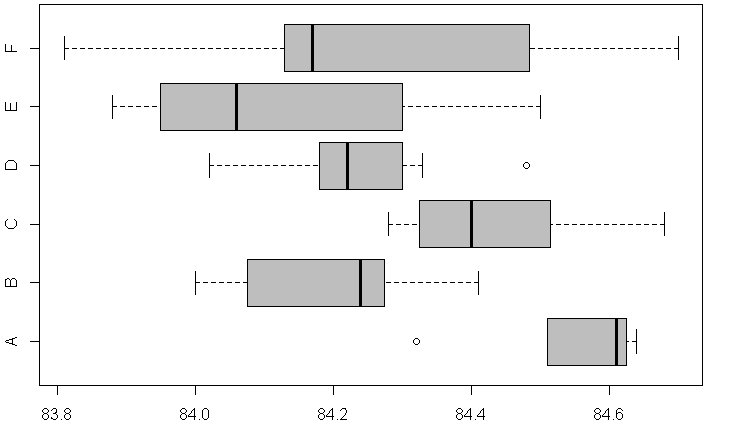
\includegraphics[scale=0.59]{ExamQ5boxplot}
\end{center}
\newpage
%qqnorm(resid(Model),pch=18,col="red",font.lab=2,font.axis=2)
%qqline(resid(Model))
\begin{center}
	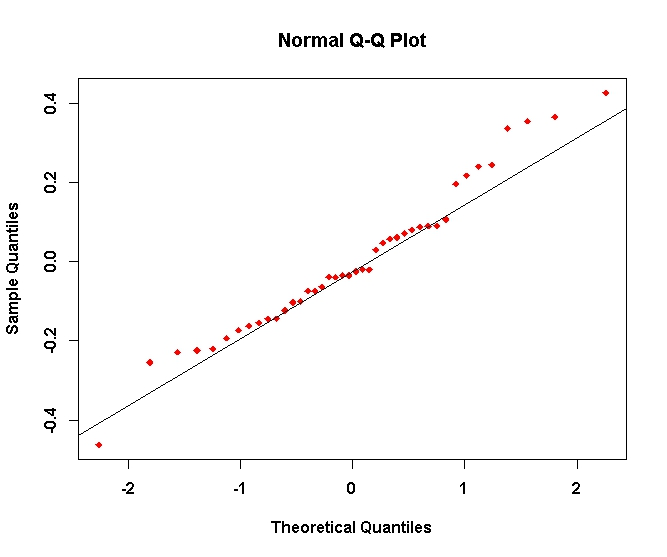
\includegraphics[scale=0.55]{ExamQ5qqplot}
\end{center}
\begin{center}
	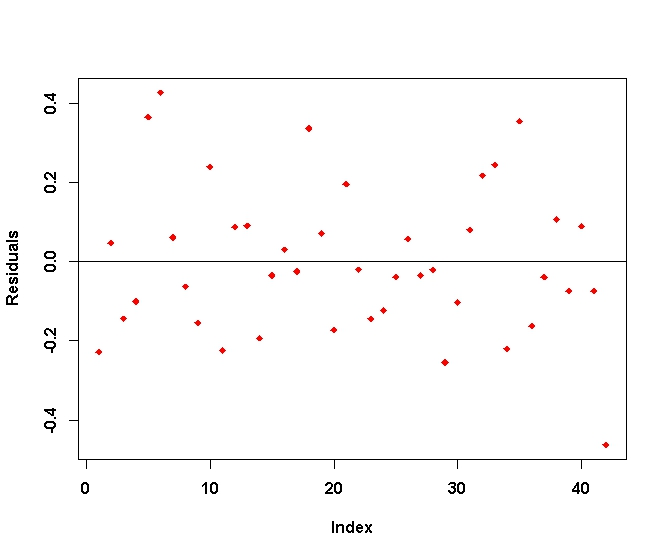
\includegraphics[scale=0.55]{ExamQ5resid}
\end{center}%
	%====================================================================== %
	\newpage
%\subsubsection*{Vegetables (ONE WAY ANOVA 4505)}
%
%(c) The following data give the recovery of bromide from spiked samples of vegetable matter, measured using a gas-liquid chromatographic method. The same amount of bromide was added to each specimen. 
%
%The units for all measurements are  mg g-1
%
%\begin{center}
%	\begin{tabular}{|c|c|c|c|}
%		Tomato: & $\{777 790 759 790 770 758 764\}$ & 774 & 142.6667
%		\\ \hline
%		
%		Cucumber: & $\{782 773 778 765 789 797 782\}$ & 781 &  106\\ \hline
%		
%		Asparagus : & $\{786 783 781 785 789 797 782 \}$& 785 & \\ \hline
%	\end{tabular} 
%\end{center}


%-------------------------------------------------------------------------------
%y<-c(777, 789, 769, 790, 770, 759, 764, 782, 774, 778, 765, 789, 
%797, 782, 785, 783, 782, 785, 787, 791, 782)
%
%
%
%T<-y[1:7];C<-y[8:14];A<-y[15:21];
%mean(T);mean(C);mean(A);
%
%-------------------------------------------------------------------------------
%-------------------------------------------------------------------------------

%
%
%\begin{itemize}
%	\item[(i)](3 Marks) Compute the Between Groups Sum of Squares, \textit{Show your workings}
%	\item[(ii)](3 Marks) Compute the Within Groups Sum of Squares, \textit{Show your workings}
%	\item[(iii)](2 Marks) Compute the Total Sum of Squares,\textit{ show your workings}
%	\item[(iv)] (2 Marks) Degrees of Fredom columns
%	\item[(v)] (1 Marks) Mean Square
%	\item[(vi)] (1 Marks) F test Statistics
%\end{itemize}
%\begin{tabular}{|c|c|c|c|c|c|}
%	\hline Source & DF & SS & MS & F & p-value \\ 
%	\hline Between &  &  &  &  &  \\ 
%	\hline Within &  &  &  &  &  \\ 
%	\hline Total &  &  &  &  &  \\ 
%	\hline 
%\end{tabular} 
%\begin{framed}
%	\begin{verbatim}
%	> bartlett.test(y~group)
%	
%	Bartlett test of homogeneity of variances
%	
%	data:  y by group
%	Bartlett's K-squared = 7.9063, df = 2, p-value = 0.01919
%	
%	\end{verbatim}
%\end{framed}

%====================================================================== %
\newpage
\subsection*{Question 3. Two Way ANOVA Procedures (25 marks) }
\subsubsection*{Question 3 Part A (6 Marks)}
%%\subsubsection*{Supermarket (TWO WAY ANOVA - MA4505)}
 A supermarket buys a particular product from four suppliers, A, B, C, D, and regular tasting tests by expert panels 
are carried out as the product is sold in their food halls. 
Various characteristics are scored and an analysis of the totals of these scores is made. 
Four tasters a, b, c, d obtained these results at four sessions 1-4.

Taster a b c d
\begin{tabular}{|c|c|c|c|c|}\hline 
&	A  & B  & C & D \\ \hline
	\hline  
	
&   21 & 17 & 18 & 20 \\
	
&	20 & 22 & 23 & 19 \\
	
&	20 & 24 & 22 & 19 \\
	
&	22 & 21 & 22 & 26 \\
	
	\hline 
\end{tabular} 



\begin{itemize}
	\item[(i.)] In the context of the above example, distinguish between the treatment and the blocking variables involved. Give reasons.
	
%	[5 marks]
	
	\item[(b)] The above data are an example of a particular experimental design. What is the general name given to this type of experimental design? Name one serious limitation of this type of experimental design.
	
%	[5 marks]
	
	\item[(c)] Complete the ANOVA table substituting the symbols ? with their correct values.
	
%	[5 marks]
	
	\item[(d)] Interpret the results.
	
%	[5 marks]
	
	\item[(e)] What is the key property of the experimental design above which allows factor effects to be estimated independently of one another. Show how this property presents itself in the above design.
	
%	[5 marks]
	
\end{itemize}
%====================================================================%
\newpage
\subsubsection*{Question 3 Part B (6 Marks)}

\begin{center}
	\texttt{
		\begin{tabular}{|cc|c|c|c|c|c|}
			\hline
			% after \\: \hline or \cline{col1-col2} \cline{col3-col4} ...
			&&		&		&		&		&		\\
			Response: Y        	&&	Df  	&	Sum Sq 	&	Mean Sq 	&	F value    	&	$Pr(>F)$    	\\
			&&	\phantom{make}	&		&		&		&		\\\hline \hline
			&&		&	\phantom{make}	&		&		&		\\
			Analyst 	&&	\textbf{?}	&	\textbf{?}	&	\textbf{?}	&	\textbf{?}	&	0.00394 **	\\
			&&		&		&		&		&		\\ \hline
			&&		&		&		&		&		\\
			Residuals	&&	\textbf{?}	&	\textbf{?}	&	0.04065	&	&		\\
			&&		&		&		&		&		\\ \hline
			&&		&		&		&		&		\\
			Total	&&	\textbf{?}	&	2.3246	&		&		&		\\
			&&		&		&		&		&		\\ \hline
		\end{tabular}
	}
\end{center}
\begin{itemize}
	\item[(i.)] (6 Marks) Complete the ANOVA table in your answer sheet, replacing the "?" entries with the correct values.\textit{\\ (You are not required to carry out a hypothesis test.)}
	%	\item[ii.] (2 marks) What hypothesis is being considered by this procedure.
	
\end{itemize}
\subsubsection*{Battery - Partial Completion ANOVA (MA4605)}

An engineer is designing a battery for use in a device that will be subjected to some extreme variations in temperature. 

The only design parameter that he can select at this point is the plate material for the battery, and he has three possible choices. 
When the device is manufactured and is shipped to the field, the engineer has no control over the temperature extremes that the device will encounter, and he knows from experience  that temperature will probably affect the effective battery life. 

However, temperature can be controlled in the product development laboratory for the purposes of a test.  The engineer decides to test all three place materials at three temperature levels – 15, 70, and 125 degrees. 

Four batteries are tested at each combination of plate material and temperature, and all 36 tests are run in random order.


The following partial ANOVA table resulted:

Analysis of Variance for Battery Life Data
%----------------------------------------------
\begin{center}
\begin{tabular}{|c|c|c|c|}\hline
	Source of & Sum of & Degrees of & Mean \\
	
	Variation & Squares & Freedom  & Square\\
	
	Material types & 2&  10,683.72 &  5,341.86 \\
	
	Temperature & 2& 39,118.72 & 19,559.36\\
	
	Interaction & 4& 9,613.78 & 2,403.44\\
	
	Error & 27& 18,230.75 & 675.21\\
	
	Total &35&77,646.97 & \\\hline
\end{tabular} 
\end{center}
% ----------------------------------------------
\begin{itemize}
\item[(i.)] Carry out appropriate tests stating clearly the null hypotheses and conclusions. 

\item[(ii.)] Would the engineer be satisfied with his design of the experiment? Explain your answer. 
\end{itemize}



\newpage
\subsubsection*{Question 3 Part C (7 Marks)}
Six analysts each made seven determinations of the paracetamol content of the same batch of tablets.
The results are shown below. There are 42 determinations in total. 
%The mean determination for each analysts is also tabulated. \\


%Analyst= structure(c(1L, 2L, 3L, 4L, 5L, 6L, 1L, 2L, 3L, 4L, 5L, 6L, 1L,
%2L, 3L, 4L, 5L, 6L, 1L, 2L, 3L, 4L, 5L, 6L, 1L, 2L, 3L, 4L, 5L,
%6L, 1L, 2L, 3L, 4L, 5L, 6L, 1L, 2L, 3L, 4L, 5L, 6L), .Label = c("A",
%"B", "C", "D", "E", "F"), class = "factor")

%Determinations= c(84.32, 84.24, 84.29, 84.14, 84.5, 84.7, 84.61, 84.13, 84.28,
%84.48, 83.91, 84.36, 84.64, 84, 84.4, 84.27, 84.11, 84.61, 84.62,
%84.02, 84.63, 84.22, 83.99, 84.15, 84.51, 84.25, 84.4, 84.22,
%83.88, 84.17, 84.63, 84.41, 84.68, 84.02, 84.49, 84.11, 84.51,
%84.3, 84.36, 84.33, 84.06, 83.81)

\begin{center}
	\begin{tabular}{|c|ccccccc|}
		\hline
		Analyst	& Content		&		&		&		&		&		&		 \\ \hline
		A	&	84.32	&	84.61	&	84.64	&	84.62	&	84.51	&	84.63	&	84.51	 \\
		B	&	84.24	&	84.13	&	84.00	&	84.02	&	84.25	&	84.41	&	84.30	 \\
		C	&	84.29	&	84.28	&	84.40	&	84.63	&	84.40	&	84.68	&	84.36	 \\
		D	&	84.14	&	84.48	&	84.27	&	84.22	&	84.22	&	84.02	&	84.33	 \\
		E	&	84.50	&	83.91	&	84.11	&	83.99	&	83.88	&	84.49	&	84.06	 \\
		F	&	84.70	&	84.36	&	84.61	&	84.15	&	84.17	&	84.11	&	83.81	 \\
		\hline
	\end{tabular}
\end{center}
\bigskip
The following \texttt{R} output has been produced as a result of analysis of these data:

%Experiment=data.frame(Determinations, Analyst)
%Model=aov(Determinations~Analyst)
%summary(Model)
\begin{framed}
	\begin{verbatim}
	Analysis of Variance Table
	
	Df   Sum Sq   Mean Sq   F value    Pr(>F)
	Analyst        5   0.8611   0.17222     4.236   0.00394 **
	Residuals     36   1.4635   0.04065
	---
	Signif. codes:  0 ‘***’ 0.001 ‘**’ 0.01 ‘*’ 0.05 ‘.’ 0.1 ‘ ’ 1
	\end{verbatim}
\end{framed}
The \texttt{R} code and graphical procedures, below and on the following page, are relevant to checking whether the underlying assumptions are met for this ANOVA model.
\begin{itemize}
	\item[(i.)] (3 Marks) What are the assumptions underlying ANOVA?
	\item[(ii.)] (4 Marks)  Assess the validity of these assumptions for the this ANOVA model.
\end{itemize}
\begin{framed}
	\begin{verbatim}
	Shapiro-Wilk normality test
	
	data:  Residuals
	W = 0.9719, p-value = 0.3819
	\end{verbatim}
\end{framed}
\begin{framed}
	\begin{verbatim}
	Bartlett test of homogeneity of variances
	
	data:  Experiment
	Bartlett's K-squared = 105.9585, df = 1, p-value < 2.2e-16
	\end{verbatim}
\end{framed}
\begin{center}
	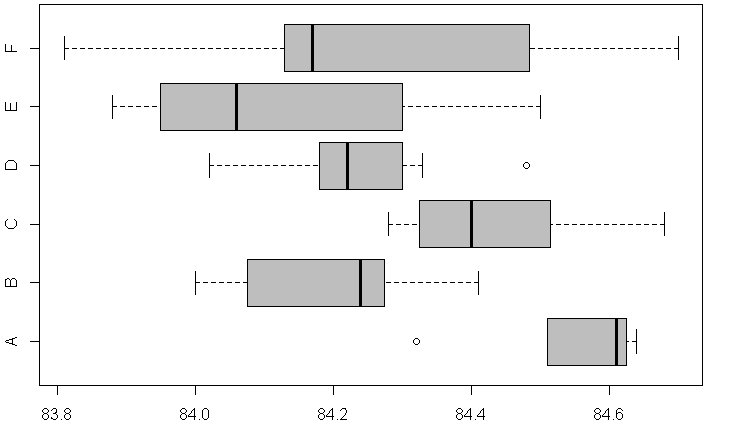
\includegraphics[scale=0.59]{ExamQ5boxplot}
\end{center}
\newpage
%qqnorm(resid(Model),pch=18,col="red",font.lab=2,font.axis=2)
%qqline(resid(Model))
\begin{center}
	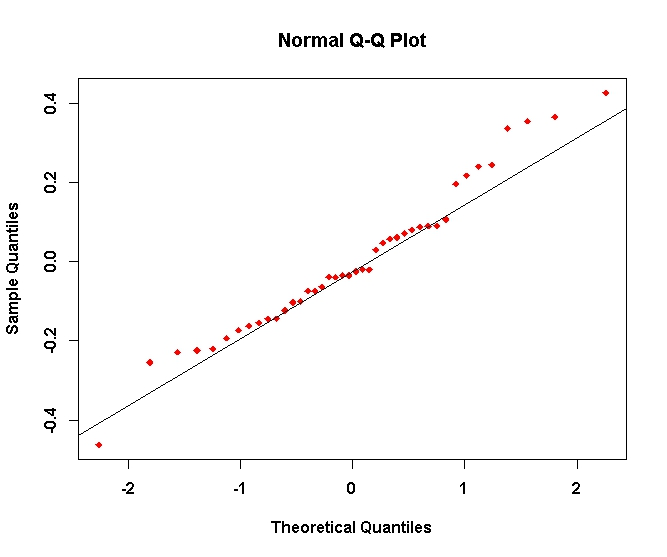
\includegraphics[scale=0.55]{ExamQ5qqplot}
\end{center}
\begin{center}
	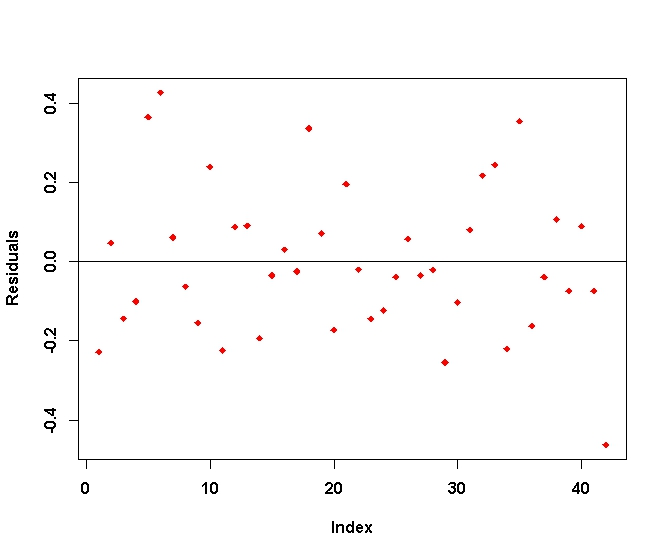
\includegraphics[scale=0.55]{ExamQ5resid}
\end{center}%
%====================================================================== %
\newpage
%\subsubsection*{Vegetables (ONE WAY ANOVA 4505)}
%
%(c) The following data give the recovery of bromide from spiked samples of vegetable matter, measured using a gas-liquid chromatographic method. The same amount of bromide was added to each specimen. 
%
%The units for all measurements are  mg g-1
%
%\begin{center}
%	\begin{tabular}{|c|c|c|c|}
%		Tomato: & $\{777 790 759 790 770 758 764\}$ & 774 & 142.6667
%		\\ \hline
%		
%		Cucumber: & $\{782 773 778 765 789 797 782\}$ & 781 &  106\\ \hline
%		
%		Asparagus : & $\{786 783 781 785 789 797 782 \}$& 785 & \\ \hline
%	\end{tabular} 
%\end{center}


%-------------------------------------------------------------------------------
%y<-c(777, 789, 769, 790, 770, 759, 764, 782, 774, 778, 765, 789, 
%797, 782, 785, 783, 782, 785, 787, 791, 782)
%
%
%
%T<-y[1:7];C<-y[8:14];A<-y[15:21];
%mean(T);mean(C);mean(A);
%
%-------------------------------------------------------------------------------
%-------------------------------------------------------------------------------

%
%
%\begin{itemize}
%	\item[(i)](3 Marks) Compute the Between Groups Sum of Squares, \textit{Show your workings}
%	\item[(ii)](3 Marks) Compute the Within Groups Sum of Squares, \textit{Show your workings}
%	\item[(iii)](2 Marks) Compute the Total Sum of Squares,\textit{ show your workings}
%	\item[(iv)] (2 Marks) Degrees of Fredom columns
%	\item[(v)] (1 Marks) Mean Square
%	\item[(vi)] (1 Marks) F test Statistics
%\end{itemize}
%\begin{tabular}{|c|c|c|c|c|c|}
%	\hline Source & DF & SS & MS & F & p-value \\ 
%	\hline Between &  &  &  &  &  \\ 
%	\hline Within &  &  &  &  &  \\ 
%	\hline Total &  &  &  &  &  \\ 
%	\hline 
%\end{tabular} 
%\begin{framed}
%	\begin{verbatim}
%	> bartlett.test(y~group)
%	
%	Bartlett test of homogeneity of variances
%	
%	data:  y by group
%	Bartlett's K-squared = 7.9063, df = 2, p-value = 0.01919
%	
%	\end{verbatim}
%\end{framed}

%====================================================================== %
\newpage
\subsection*{Question 4. Linear Models (25 Marks)}
\subsubsection*{Question 4 Part A (12 Marks)}
The mercury level of several tests of sea-water from costal areas was determined by atomic-absorption spectrometry. The results obtained are as follows

\begin{figure}[h!]
	\centering
	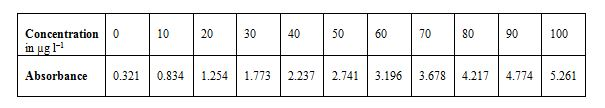
\includegraphics[width=1.1\linewidth]{image/regressionData}
\end{figure}

The analysis of the relationship between concentration and absorbance is obtained in R and presented below. 
\begin{framed}
	\begin{verbatim}
	x<-seq(0,100,by=10)
	y<- c(0.321, 0.834, 1.254, 1.773, 2.237, 2.741, 3.196, 3.678, 
	4.217, 4.774, 5.261)
	model<- lm(y~x)
	summary(model)
	
	Call:
	lm(formula = y ~ x)
	
	Coefficients:
	Estimate Std. Error t value Pr(>|t|)    
	(Intercept) 0.2933636  0.0234754   12.50 5.45e-07 
	x           0.0491982  0.0003968  123.98 7.34e-16 
	---
	
	Residual standard error: 0.04162 on 9 degrees of freedom
	Multiple R-squared: 0.9994,     Adjusted R-squared: 0.9993 
	F-statistic: 1.537e+04 on 1 and 9 DF,  p-value: 7.337e-16 
	
	confint(model)
	2.5 %     97.5 %
	(Intercept) 0.24025851 0.34646876
	x           0.04830054 0.05009582
	
	\end{verbatim}
\end{framed}
\newpage
\begin{itemize}
	\item[(i)] (2 marks)
	Determine and interpret the slope and the intercept of the regression line.
	\item[(ii)]  (2 marks) State the 95\% confidence interval for the slope and the intercept coefficients. Interpret this intervals with respect to any relevant hypothesis tests
	\item[(iii)] (2 marks) Explain in which way is the prediction intervals different from the confidence intervals for fitted values in linear regression?
	\item[(iv)] (2 Marks) The following piece of \texttt{R} code gives us a statistical metric. What is this metric? What is it used for? How should it be interpreted.
	
\end{itemize}
\begin{framed}
	\begin{verbatim}
	> AIC(model)
	[1] -34.93389	
	\end{verbatim}
\end{framed}

%=====================================================

%Write a short note to compare and contrast the multiple R squared and asjusted R squared.
%%% - Overfitting
	
%====================================================================== %
	\newpage

\subsubsection*{Question 4 Part B (12 Marks)}

%\subsubsection*{Model Selection}
Given the AIC for each candidate model, use \textbf{\textit{Backward Selection}} to determine the optimal model for predicting values of $y$ with predictor variables
$x_1$, $x_2$,$x_3$ and $x_4$.

 Suppose we have 5 predictor variables.
Use \textbf{Forward Selection} and \textbf{Backward Selection} to choose the optimal set of predictor variables, based on the AIC measure.

{
	\large
	\begin{center}
		\begin{tabular}{||c|c||c|c||}
			\hline
			Variables & AIC & Variables & AIC \\ \hline \hline
			$\emptyset$	&	200	&	x1, x2, x3	&	74	\\ \hline
			\phantom{makemakespace}
			&	\phantom{makespace}
			&	x1, x2, x4	&	75	\\ \hline
			x1	&	150	&	x1, x2, x5	&	79	\\ \hline
			x2	&	145	&	x1, x3, x4	&	72	\\ \hline
			x3	&	135	&	x1, x3, x5	&	85	\\ \hline
			x4	&	136	&	x1, x4, x5	&	95	\\ \hline
			x5	&	139	&	x2, x3, x4	&	83	\\ \hline
			&		&	x2, x3, x5	&	82	\\ \hline
			x1, x2	&	97	&	x2, x4, x5	&	78	\\ \hline
			x1, x3	&	81	&	x3, x4, x5	&	85	\\ \hline
			x1, x4	&	94	&	\phantom{makemakespace}
			&	\phantom{makespace}
			\\ \hline
			x1, x5	&	88	&	x1, x2, x3, x4	&	93	\\ \hline
			x2, x3	&	87	&	x1, x2, x3, x5	&	120	\\ \hline
			x2, x4	&	108	&	x1, x2, x4, x5	&	104	\\ \hline
			x2, x5	&	87	&	x1, x3, x4, x5	&	101	\\ \hline
			x3, x4	&	105	&	x2, x3, x4, x5	&	89	\\ \hline
			x3, x5	&	82	&		&		\\ \hline
			x4, x5	&	86	&	x1, x2, x3, x4, x5	&	100	\\ \hline
		\end{tabular} 
	\end{center}
}
%================================================= %
\newpage
%\subsubsection*{Regression ANOVA}
\subsubsection*{Question 3 Part B (6 Marks)}
Suppose we have a regression model, described by the following equation
\[ \hat{y} = 28.81 + 6.45x_1 + 7.82 x_2\]
We are given the following pieces of information.
\begin{itemize}
	\item The standard deviation of the response variance $y$ is 10 units.
	\item There are 53 observations.
	\item The \textit{Coefficient of Determination} (also known as the \textit{Multiple R-Squared}) is 0.75.
\end{itemize}
Complete the \textit{Analysis of Variance} Table for a linear regression model.
The required values are indicated by question marks.

\begin{center}
	\begin{tabular}{|c|c|c|c|c|c|} \hline
	\phantom{makespace}	& DF & 	Sum Sq &	Mean Sq &	F value &   	Pr($>$F)    \\ \hline
		Regression &  \phantom{make}?\phantom{make} &	? &	? &	 ? &	$< 2.2e^{-16}$ \\ \hline
		Error  & ? &	? &  	?   &            &       \\ \hline
		Total  & ?  &	? &  \phantom{makespace}	  &   \phantom{makespace}         &    \phantom{makespace}    \\ \hline
	\end{tabular} 
\end{center}


\newpage
%======================================================


\subsection*{Question 5. Statistical Process Control (25 marks) }

\subsubsection*{Question 5 Part A (12 Marks)}
% \subsection*{Question 47 - Nelson Rules for Control Charts}
The \textbf{Nelson Rules} are a set of eight decision rules for detecting ``out-of-control" or non-random conditions on control charts. These rules are applied to a control chart on which the magnitude of some variable is plotted against time. The rules are based on the mean value and the standard deviation of the samples.\\

\begin{itemize}
	\item[(i)] ($4 \times 2$ Marks) Discuss any four of these rules, and how they would be used to detect ``out of control" processes. Support your answer with sketch.
\end{itemize}

\bigskip 
\begin{framed}
	\noindent \textit{In your answer, you may make reference to the following properties of the Normal Distribution. Consider the random variable $X$ distributed as
		\[X \sim \mathcal{N}(\mu,\sigma^2)\]
		where $\mu$ is the mean and $\sigma^2$ is the variance of an random variable $X$.}
	\begin{itemize}
		\item $\Pr( \mu - 1\sigma \leq X \leq \mu + 1\sigma ) = 0.6827$
		\item $\Pr( \mu - 2\sigma \leq X \leq \mu + 2\sigma ) = 0.9545$
		\item $\Pr( \mu - 3\sigma \leq X \leq \mu + 3\sigma )= 0.9973$
		
	\end{itemize}
\end{framed}
\newpage

\subsubsection*{Question 5 Part B (6 Marks)}
A normally distributed quality characteristic is monitored through the use of control charts. These charts have the following parameters. All charts are in control.
\begin{center}
	\begin{tabular}{|c|c|c|c|}
		\hline  & LCL & Centre Line & UCL \\
		\hline $\bar{X}$-Chart & 1995 & 2000 & 2005 \\
		\hline $R$-Chart & 0 & 21 & 44.394 \\ \hline
	\end{tabular}
\end{center}

\begin{itemize}
	\item[(i.)] (2 Marks) What sample size is being used for this analysis?
	\item[(ii.)] (2 Marks) Estimate the mean of the process standard deviations $\bar{s}$.
	\item[(iii.)] (2 Marks) Compute the control limits for the process standard deviation chart (i.e. the s-chart).
\end{itemize}


\subsubsection*{Question 5 Part C (7 Marks)}
An automobile assembly plant concerned about quality improvement measured sets of five camshafts on twenty occasions throughout the day. The specifications for the process state that the design specification limits at 600$\pm$3mm.


\begin{itemize}
	\item[(i.)] (4 Marks) Determine the \emph{Process Capability Indices} $C_p$ and $C_{pk}$, commenting on the respective values. Use the \texttt{R} code output on the following page.
	\item[(ii.)] (2 Mark)  Explain why there would be a discrepancy between $C_p$ and $C_{pk}$. Illustrate your answer with sketches.
	\item[(iii.)] (1 Mark) Comment on the graphical output of the \emph{Process Capability Analysis}, also presented on the next page.
\end{itemize}



\newpage
\begin{framed}
	\begin{verbatim}
	Process Capability Analysis
	
	Call:
	process.capability(object = obj,  
	spec.limits = c(597, 603))
	Number of obs = 100          Target = 600
	Center = 599.548         LSL = 597
	StdDev = 0.5846948       USL = 603
	
	Capability indices:
	Value   2.5%  97.5%
	Cp    ...
	Cp_l  ...
	Cp_u  ...
	Cp_k  ...
	Cpm   1.353  1.134  1.572
	Exp<LSL 0%   Obs<LSL 0%
	\end{verbatim}
\end{framed}



\begin{center}
	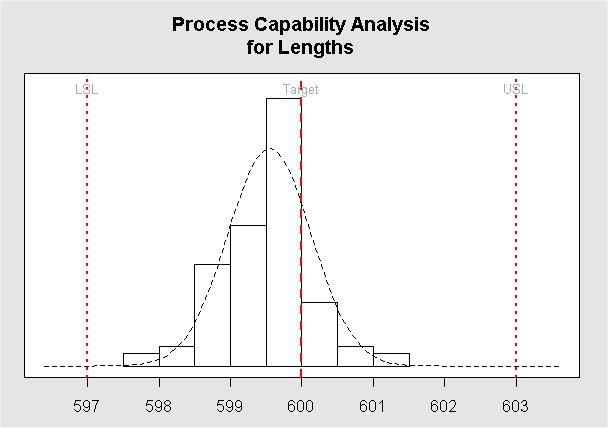
\includegraphics[scale=0.55]{image/ExamQ4hist}
\end{center}
\newpage
%
%Lengths = Values
%
%obj <- qcc(Lengths, type="xbar")
%
%process.capability(obj, spec.limits=c(597,603))

\section*{Formulas and Tables}

	\subsection*{Critical Values for Dixon Q Test}
	{
		\Large
		\begin{center}
			\begin{tabular}{|c|c|c|c|}
				\hline  N  & $\alpha=0.10$  & $\alpha=0.05$  & $\alpha=0.01$  \\ \hline
				3  & 0.941 & 0.97  & 0.994 \\ \hline
				4  & 0.765 & 0.829 & 0.926 \\ \hline
				5  & 0.642 & 0.71  & 0.821 \\ \hline
				6  & 0.56  & 0.625 & 0.74  \\ \hline
				7  & 0.507 & 0.568 & 0.68  \\ \hline
				8  & 0.468 & 0.526 & 0.634 \\ \hline
				9  & 0.437 & 0.493 & 0.598 \\ \hline
				10 & 0.412 & 0.466 & 0.568 \\ \hline
				11 & 0.392 & 0.444 & 0.542 \\ \hline
				12 & 0.376 & 0.426 & 0.522 \\ \hline
				13 & 0.361 & 0.41  & 0.503 \\ \hline
				14 & 0.349 & 0.396 & 0.488 \\ \hline
				15 & 0.338 & 0.384 & 0.475 \\ \hline
				16 & 0.329 & 0.374 & 0.463 \\ \hline
			\end{tabular} 
		\end{center}
	}
	\subsection*{Critical Values for Chi Square Test}
	{
		\Large
		\begin{center}
			\begin{tabular}{|c|c|c|c|c|}
				\hline 
				n	&	$\alpha=0.10$	&	$\alpha=0.05$	&	$\alpha=0.01$	&	$\alpha=0.001$	\\ \hline
				1	& 	2.705	&	3.841	&	6.634	&	10.827	\\ \hline
				2	&	4.605	&	5.991	&	7.378	&	9.21	\\ \hline
				3	&	6.251	&	7.815	&	9.348	&	11.345	\\ \hline
				4	&	7.779	&	9.488	&	11.143	&	13.277	\\ \hline
				5	&	9.236	&	11.07	&	12.833	&	15.086	\\ \hline
				6	&	10.645	&	12.592	&	14.449	&	16.812	\\ \hline
				7	&	12.017	&	14.067	&	16.013	&	18.475	\\ \hline
				8	&	13.362	&	15.507	&	17.535	&	20.09	\\ \hline
				9	&	14.684	&	16.919	&	19.023	&	21.666	\\ \hline
				10	&	15.987	&	18.307	&	20.483	&	23.209	\\ \hline
			\end{tabular} 
		\end{center}
	}
\newpage

\subsection*{Two Way ANOVA}
\[MS_A = c \times S^2_r\]
\[MS_B = r \times S^2_c\]

\subsection*{Control Limits for Control Charts}

\[ \bar{\bar{x}} \pm 3\frac{\bar{s}}{c_4\sqrt{n}}\]

\[ \bar{s} \pm 3\frac{c_5\bar{s}}{c_4}\]

\[\left[ \bar{R}D_3, \bar{R}D_4\right]\]

\subsection*{Process Capability Indices}
\[ \hat{C}_p = \frac{\mbox{USL} - \mbox{LSL}}{6s}\]

\[ \hat{C}_{pk} = \mbox{min} \left[\frac{\mbox{USL} - \bar{x}}{3s},\frac{\bar{x} - \mbox{LSL}}{3s} \right] \]

\[ \hat{C}_{pm} = \frac{\mbox{USL} - \mbox{LSL}}{6\sqrt{s^2+(\bar{x}-T)^2}}\]
\bigskip
	\newpage
	
	%------------------------------------------------------------------------ %
	\Large{
		\subsection*{Factors for Control Charts}
		\begin{tabular}{|c|c|c|c|c|c|c|}
			\hline
			Sample Size (n) 	&	c4 	&	c5 	&	d2 	&	d3 	&	D3 	&	D4	\\	\hline
			2	&	0.7979	&	0.6028	&	1.128	&	0.853	&	0	&	3.267	\\	
			3	&	0.8862	&	0.4633	&	1.693	&	0.888	&	0	&	2.574	\\	
			4	&	0.9213	&	0.3889	&	2.059	&	0.88	&	0	&	2.282	\\	
			5	&	0.9400	&	0.3412	&	2.326	&	0.864	&	0	&	2.114	\\	
			6	&	0.9515	&	0.3076	&	2.534	&	0.848	&	0	&	2.004	\\	
			7	&	0.9594	&	0.282	&	2.704	&	0.833	&	0.076	&	1.924	\\	
			8	&	0.9650	&	0.2622	&	2.847	&	0.82	&	0.136	&	1.864	\\	
			9	&	0.9693	&	0.2459	&	2.970	&	0.808	&	0.184	&	1.816	\\	
			10	&	0.9727	&	0.2321	&	3.078	&	0.797	&	0.223	&	1.777	\\	
			11	&	0.9754	&	0.2204	&	3.173	&	0.787	&	0.256	&	1.744	\\	
			12	&	0.9776	&	0.2105	&	3.258	&	0.778	&	0.283	&	1.717	\\	
			13	&	0.9794	&	0.2019	&	3.336	&	0.770	&	0.307	&	1.693	\\	
			14	&	0.9810	&	0.1940	&	3.407	&	0.763	&	0.328	&	1.672	\\	
			15	&	0.9823	&	0.1873	&	3.472	&	0.756	&	0.347	&	1.653	\\	
			16	&	0.9835	&	0.1809	&	3.532	&	0.750	&	0.363	&	1.637	\\
			17	&	0.9845	&	0.1754	&	3.588	&	0.744	&	0.378	&	1.622	\\
			18	&	0.9854	&	0.1703	&	3.64	&	0.739	&	0.391	&	1.608	\\
			19	&	0.9862	&	0.1656	&	3.689	&	0.734	&	0.403	&	1.597	\\
			20	&	0.9869	&	0.1613	&	3.735	&	0.729	&	0.415	&	1.585	\\
			21	&	0.9876	&	0.1570	&	3.778	&	0.724	&	0.425	&	1.575	\\
			22	&	0.9882	&	0.1532	&	3.819	&	0.720	&	0.434	&	1.566	\\
			23	&	0.9887	&	0.1499	&	3.858	&	0.716	&	0.443	&	1.557	\\
			24	&	0.9892	&	0.1466	&	3.895	&	0.712	&	0.451	&	1.548	\\
			25	&	0.9896	&	0.1438	&	3.931	&	0.708	&	0.459	&	1.541	\\
			\hline
		\end{tabular}
	} % End Large Font
	
\end{document}

Outliers
Boxplots Outliers ( Upper Fence Lower Fence)
Dixon Q-Test
%----------------------------------%
Chi Square 12 Marks
%=====================================================





%========================================================%

\section{R Code for Part 3}
\begin{verbatim}
ALL <- c(84.32, 84.51, 84.63, 84.61, 84.64, 84.51, 84.62, 84.24, 84.25, 
84.41, 84.13, 84, 84.3, 84.02, 84.29, 84.4, 84.68, 84.28, 84.4, 
84.36, 84.63, 84.14, 84.22, 84.02, 84.48, 84.27, 84.33, 84.22, 
84.5, 83.88, 84.49, 83.91, 84.11, 84.06, 83.99, 84.7, 84.17, 
84.11, 84.36, 84.61, 83.81, 84.15)

\end{verbatim}
%==================================================%
library(xtable)

nu1 <- 2:10
nu2 <- c(5:15,18,21,24,27,30)

L1 <- length(nu1)
L2 <- length(nu2)
CVs <- matrix(ncol=L1,nrow=L2)


for( i in 1:L2){
	for( j in 1:L1){ 
		CVs[i,j] <- round( qf(0.95,i,j),3)
	}
	
}

colnames(CVs)<- nu1

rownames(CVs)<- nu2

xtable(CVs) 

%======================================================================= %
Dixon

chi Square

Normal

One Way ANOVA

Two Way ANOVA interactions

Test Normality

SPC definitions





min=23
max=89
range=65
gap=31
TS =31/65 = 0.47692
CV =0.396 (5\%)
Reject Ho


